\documentclass{article}
\usepackage[ backend=biber]{biblatex}
\addbibresource{proposal/prop.bib}
\ExecuteBibliographyOptions{sorting=none,maxbibnames=5,doi=false,isbn=false,url=false}
\usepackage{fullpage}
\usepackage[utf8]{inputenc}
\usepackage{amsmath}
\usepackage{amssymb}
\usepackage{amsthm}
\usepackage{mathrsfs}
\usepackage{bbold}
\usepackage{wesa}
\usepackage{graphicx}
\usepackage{verbatim}

\theoremstyle{remark}
\newtheorem{example}{Example}
\newtheorem{definition}{Definition}
\newtheorem{thm}{Theorem}
\newtheorem{lemma}{Lemma}

\newcommand{\Hilb}{\mathcal{H}}
\newcommand{\events}{\ensuremath{\mathcal{E}}}
\newcommand{\qevents}{\ensuremath{\mathcal{E}}}
\newcommand{\pmeas}{\ensuremath{\mu}}
\newcommand{\imposs}{{\mbox{\wesa{impossible}}}}
\newcommand{\likely}{{\mbox{\wesa{likely}}}}
\newcommand{\unlikely}{{\mbox{\wesa{unlikely}}}}
\newcommand{\necess}{{\mbox{\wesa{certain}}}}
\newcommand{\unknown}{{\mbox{\wesa{unknown}}}}
\newcommand{\ket}[1]{{\left\vert{#1}\right\rangle}}
\newcommand{\op}[2]{\ensuremath{\left\vert{#1}\middle\rangle\middle\langle{#2}\right\vert}}
\newcommand{\proj}[1]{\op{#1}{#1}}
\newcommand{\ps}{\texttt{+}}
\newcommand{\ms}{\texttt{-}}
\newcommand{\ip}[2]{\ensuremath{\left\langle{#1}\middle\vert{#2}\right\rangle}}
\newcommand{\Tr}{\mathop{\mathrm{Tr}}\nolimits}
\newcommand{\rme}{\mathrm{e}}
\newcommand{\rmi}{\mathrm{i}}

\usepackage{color}
\usepackage[usenames,dvipsnames]{xcolor}
\newcommand{\amr}[1]{\fbox{\begin{minipage}{0.9\textwidth}\color{green}{Amr says: #1}\end{minipage}}}
\newcommand{\yutsung}[1]{\fbox{\begin{minipage}{0.9\textwidth}\color{purple}{Yu-Tsung says: #1}\end{minipage}}}
\newcommand{\set}[2]{\ensuremath{\left\{ {#1}~\middle|~{#2}\right\} }}

\begin{document}
\title{Measurement and Probability in Fuzzy Quantum Theories}
\date{\today}
\maketitle 

%%%%%%%%%%%%%%%%%%%%%%%%%%%%%%%%%%%%%%%%%%%%%%%%%%%%%%%%%%%%%%%%%%%%%%%%%%%%%%
\section{Introduction}

This is a \emph{theoretical} investigation of \emph{experimental}
physics using \emph{computational} methods. All experiments and computations
are processes bounded in space, time, energy, and other resources~\cite{Jaeger2007,Piccinini2015}.
Yet, for centuries, the mathematical formalization of such processes
has been founded on the infinitely precise real or complex numbers~\cite{Ziegler2007,weihrauch2012computable,blum2012complexity}.
Our purpose here is to exploit the consequences of replacing infinitely-specified
quantum probabilities by finite number of intervals used in interval-valued
probability measures~(IVPM); in particular, we show that a quantum
IVPM may not be induced by a infinitely-precise state, but it might
be more and more likely to be identified to a particular state when
the measurement resources increase.

Indeed, almost every description of quantum mechanics, quantum computation,
or quantum experiments refers to entities such as $\rme$, $\pi$,
$\sqrt{2}$, etc (see, e.g., \cite{Redhead1987-REDINA,544199,Mermin2007}).
From a computational perspective, such numbers do not exist in their
entirety ``for free~\cite{Kent1999,CliftonKent2000}.'' For example,
the state of the art algorithms for computing the $n$th binary digit
of~$\pi$ require on the order of $O\left(n\log^{O\left(1\right)}\left(n\right)\right)$
operations~\cite{journals/moc/BaileyBP97}. In other words, simply
referring to the $n$th digit of $\pi$ requires more and more resources
as $n$ gets larger. Taking such resource bounds into consideration
is what founded computer science as a discipline and is crucial for
understanding the very nature of computation and, following Feynman~\cite{Feynman1982Simulating},
Landauer~\cite{Landauer1996188}, and others, for understanding the
very nature of physical processes.

We have been revisiting quantum mechanics, quantum information, and
quantum computation from this resource-aware perspective. Our initial
results in that domain showed how subtle the issues can be~\cite{usat,geometry2013,DQT2014}:
a straightforward replacement of the complex numbers by a finite field
yields a variant of quantum mechanics in which computationally hard
problems like UNIQUE-SAT (which decides whether a given Boolean formula
is unsatisfiable or has exactly one satisfying assignment~\cite{Valiant198685,Papadimitriou1993,AroraBarak2009})
can be deterministically solved in constant time. To eliminate such
unrealistic theories requires delicate analysis of the structure of
the Hilbert space, the process of observation, and the notion of probability
teasing apart their reliance on the infinitely precise real numbers~\cite{geometry2013,DQT2014}. 

In this paper, we shift focus from the infinitely-specified but not
directly observable quantum states, to observable measurable properties
of quantum systems and their probabilities. Furthermore, we insist
that our theories of measurement and probability only refer to finitely
communicable evidence within feasible computational bounds. It follows
that states, observations, and probabilities all become ``fuzzy'',
i.e., specified by intervals of confidence that can only increase
in precision if the available resources increase proportionally. Our
notion of ``fuzzy quantum mechanics'' is related to existing work~\cite{GranikCaulfield1996,Pykacz2013,SNL2009,Gudder2005,aerts1993physical}
but, as will be explained in more detail, is distinguished by its
unique computational character.

We will begin by reviewing existing work that recasts classical probability
spaces in a resource-aware setting and move to aim at recasting quantum
probability and quantum measurement. In particular, we develop a measurement
framework based on quantum IVPM. Surprisingly, we found a quantum
IVPM which can not be induced by a state, while Shapley proved a classical
convex IVPM can always be induced by a classical ``state''~\cite{Shapley1971,Grabisch2016},
and Gleason proved a infinitely-specified quantum probabilities measure
can always be induced by a quantum state~\cite{gleason1957,Redhead1987-REDINA,peres1995quantum}.
Nevertheless, a quantum IVPM could still correspond to many possible
states if it is broken into pieces. Our examples also suggest that
a quantum IVPM could be more and more likely induced by a state while
the intervals become sharper, i.e., the measurement resources increase.

Since Gleason's theorem supports the idea of von Neumann to define
a state as a density matrix~\cite{Varadarajan2008}, a density matrix
might not be a adequate imprecise quantum state. Instead, a imprecise
quantum state might be more like an interactive system suggested by
Quantum Bayesianism or QBism~\cite{Fuchs2010,VonBaeyer2016,Fuchs2012},
which would interact differently with different clients. Furthermore,
the validity the fundamental theorems of quantum mechanics followed
up by Gleason's theorem, such as Bell~\cite{BellBook1987,Redhead1987-REDINA,peres1995quantum,Jaeger2007}
and Kochen-Specker~\cite{kochenspecker1967,Redhead1987-REDINA,peres1995quantum,Jaeger2007},
might need to be reassessed based on our imprecise measurement. Our
research then might provide a new insight to the old debate among
Meyer, Mermin, and others about  whether finite precision measurement
would nullify the Kochen-Specker theorem or not~\cite{PhysRevLett.83.3751,Mermin1999,BarrettKent2004}.

%%%%%%%%%%%%%%%%%%%%%%%%%%%%%%%%%%%%%%%%%%%%%%%%%%%%%%%%%%%%%%%%%%%%%%%%%%%%%%
\section{Classical Probability}

A \emph{probability space} specifies the necessary conditions for
reasoning coherently about collections of uncertain
events~\cite{Kolmogorov1950,Shafer1976,Griffiths2003,Swart2013}.  We
review the conventional presentation of probability spaces and then
discuss the computational resources needed to estimate probabilities.

%%%
\subsection{Classical Probability Spaces}

The conventional definition of a probability space builds upon the
field of real numbers. In more detail, a probability space consists
of a \emph{sample space} $\Omega$, a space of \emph{events}~$\events$,
and a \emph{probability measure}~$\pmeas$ mapping events in $\events$
to the real interval $[0,1]$. We will only consider \emph{finite}
sets of events and restrict our attention to non-empty finite sets
$\Omega$ as the sample space. The space of events $\events$ includes
every possible subset of $\Omega$: it is the powerset~$2^{\Omega}=\set{E}{E\subseteq\Omega}$.
For future reference, we emphasize that events are the primary notion
of interest and that the sample space is a convenient artifact that
allows us to treat events as sets obeying the laws of Boolean algebra~\cite{Boole1948,Redhead1987-REDINA,Griffiths2003}.

\begin{definition}[Probability Measure]\label{def:ClassicalProbabilitySpace}
  Given the set of events $\events$, a \emph{probability measure} is a
  function $\pmeas:\events\rightarrow[0,1]$ such that:
\begin{itemize}
\item $\pmeas(\emptyset)=0$,
\item $\pmeas(\Omega)=1$, 
\item for every event $E$,
  $\pmeas\left(\Omega\backslash E\right)=1-\pmeas\left(E\right)$ where
  $\Omega\backslash E$ is the complement event of $E$, and
\item for every collection $\left\{ E_{i}\right\} _{i=1}^{N}$ of
  pairwise disjoint events,
  $\pmeas\left(\bigcup_{i=1}^{N}E_{i}\right)=\sum_{i=1}^{N}\pmeas(E_{i})$.
\end{itemize}
\end{definition}
\noindent There is some redundancy in the definition that will be useful when
moving to quantum probability spaces. 

\begin{example}[Two-coins experiment]\label{ex1} Consider an
  experiment that tosses two coins. We have four possible outcomes
  that constitute the sample space $\Omega=\{HH,HT,TH,TT\}$. There are
  16 total events including the event $\{HH,HT\}$ that the first coin
  lands heads up, the event $\{HT,TH\}$ that the two coins land on
  opposite sides, and the event $\{HT,TH,TT\}$ that at least one coin
  lands tails up. Here is a possible probability measure for these
  events:
\[
\begin{array}{c@{\qquad\qquad}c}
\begin{array}{rcl}
\pmeas(\emptyset) & = & 0\\
\pmeas(\{HH\}) & = & 1/3\\
\pmeas(\{HT\}) & = & 0\\
\pmeas(\{TH\}) & = & 2/3\\
\pmeas(\{TT\}) & = & 0\\
\pmeas(\{HH,HT\}) & = & 1/3\\
\pmeas(\{HH,TH\}) & = & 1\\
\pmeas(\{HH,TT\}) & = & 1/3
\end{array} & \begin{array}{rcl}
\pmeas(\{HT,TH\}) & = & 2/3\\
\pmeas(\{HT,TT\}) & = & 0\\
\pmeas(\{TH,TT\}) & = & 2/3\\
\pmeas(\{HH,HT,TH\}) & = & 1\\
\pmeas(\{HH,HT,TT\}) & = & 1/3\\
\pmeas(\{HH,TH,TT\}) & = & 1\\
\pmeas(\{HT,TH,TT\}) & = & 2/3\\
\pmeas(\{HH,HT,TH,TT\}) & = & 1
\end{array}\end{array}
\]
\end{example}

\noindent It is useful to think that this probability measure is
completely determined by the ``reality'' of the two coins in question
and their characteristics, in the sense that each pair of coins
induces a measure, and each measure must correspond to some pair of
coins. The measure above would be induced by two particular coins such
that the first coin is twice as likely to land tails up than heads up
and the second coin is double-headed. In a strict computational
or experimental setting, one should question the reliance of the
definition of probability space on the uncountable and
uncomputable real
interval~$[0,1]$~\cite{Turing_1937,Ziegler2007,weihrauch2012computable}.
This interval includes numbers like
$0.h_{1}h_{2}h_{3}\ldots$ where $h_{i}$ is 1 or 0 depending on whether
Turing machine $\mathit{TM}_{i}$ halts or not. Such numbers cannot be
computed. This interval also includes numbers like $\frac{\pi}{4}$
which can only be computed with increasingly large resources as the
precision increases. Therefore, in a resource-aware computational or
experimental setting, it is more appropriate to consider probability
measures that map events to a set of elements computable with a fixed
set of resources. We expand on this observation in the next section
and then recall its formalization using interval-valued probability
measures~\cite{Weichselberger2000,JamisonLodwick2004}.

%%%%%
\subsection{Measuring Probabilities: Buffon's Needle Problem\label{subsec:Measuring-Probabilities:-Buffon}}

In the previous example, we assumed the probability~$\pmeas(E)$ of
each event~$E$ is known a priori. In reality, although each event is
assumed to have a probability, the exact value of $\pmeas(E)$ may not
be known. According to the \emph{frequency interpretation of
  probability} (which we will revisit when moving to the quantum
case)~\cite{Venn1876,Hajek2012}, 
to determine the probability of an event, we run $M$
independent trials which gives us an approximation of the (assumed)
``true'' or ``real'' probability. Let $x_{i}$ be 1 or 0 depending on
whether the event~$E$ occurs in the $i$-th trial or not, then
$\pmeas(E)$ could be approximated to given accuracy~$\epsilon>0$ by
the relative frequency~$\frac{1}{M}\sum_{i=1}^{M}x_{i}$ with the
probability converging to one as $M$ goes to infinity, i.e.,
\[
\forall\epsilon>0,\lim_{M\rightarrow\infty}\pmeas\left(\left|\pmeas(E)-\frac{1}{M}\sum_{i=1}^{M} x_{i}\right|<\epsilon\right)=1\textrm{ .}
\]
This fact is called the law of large numbers~\cite{Bernoulli2006,Kolmogorov1950,Uspensky1937,Shafer1976,544199}.

Let's look at a concrete example. Suppose we drop a needle of length
$\ell$ onto a floor made of equally spaced parallel lines a distance
$h$ apart, where $\ell<h$. It is a known fact that the probability of
the needle crossing a line is
$\frac{2\ell}{\pi
  h}$~\cite{Buffon1777,DeMorgan1872,Hall1873,Uspensky1937}.
Consider an experimental setup consisting of a collection of $M$
identical needles of length $\ell$. We throw the $M$ needles one
needle at a time, and observe the number $M_c$ of needles that cross a
line, thus estimating the probability of a needle crossing a line to
be $\frac{M_c}{M}$. In an actual experiment with $500$ needles and the
ratio $\frac{\ell}{h}=0.75$~\cite{Hall1873}, it was found that $236$
crossed a line so the relative frequency is $0.472$ whereas the
idealized mathematical probability is $0.4774\ldots$.  In a larger
experiment with $5000$ needles and the ratio
$\frac{\ell}{h}=0.8$~\cite{Uspensky1937}, the relative frequency was
calculated to be $0.5064$ whereas the idealized mathematical
probability is $0.5092\ldots$. We see that the observed probability
approaches $\frac{2\ell}{\pi h}$ but only if \emph{larger and larger
  resources} are expended. These resource considerations suggest that
it is possible to replace the real interval $[0,1]$ with rational
numbers up to a certain precision related to the particular experiment
in question. There is clearly a connection between the number of
needles and the achievable precision: in the hypothetical experiment
with 3 needles, it is not sensible to retain 100 digits in the
expansion of $\frac{2\ell}{\pi h}$.

There is another more subtle assumption of unbounded computational
power in the experiment. We are assuming that we can always determine
with certainty whether a needle is crossing a line. But ``lines'' on
the the floor have thickness, their distance apart is not exactly $h$,
and the needles' lengths are not all absolutely equal to $\ell$.
These perturbations make the events ``fuzzy.'' Thus, in an experiment
with limited resources, it is not possible to talk about the idealized
event that exactly $M_c$ needles cross lines as this would require the
most expensive needles built to the most precise accuracy, laser
precision for drawing lines on the floor, and the most powerful
microscopes to determine if a needle does cross a line. Instead we
might talk about the event that $M_c-\delta$ needles evidently cross
lines and $M_c+\delta'$ needles plausibly cross lines where $\delta$ and
$\delta'$ are resource-dependent approximations. This fuzzy notion of
events leads to probabilities being only calculable within intervals
of confidence reflecting the certainty of events and their
plausibility. This is indeed consistent with published experiments: in
an experiment with $3204$ needles and the ratio
$\frac{\ell}{h}=0.6$~\cite{DeMorgan1872}, $1213$ needles clearly
crossed a line and $11$ needles were close enough to plausibly be
considered as crossing the line: we would express the probability in
this case as the interval
$\left[\frac{1213}{3204},\frac{1224}{3204}\right]$ expressing that we
are certain that the event has probability at least
$\frac{1213}{3204}$ but it is possible that it would have probability
$\frac{1224}{3204}$.

\amr{Another: the calculus of probabilities requires all probabilities to
be \emph{coherent}. But given limited resources, a user can only
approximate the probabilities and the approximation may not be
completely coherent in the ideal sense.}

%%%%%
\subsection{Classical Interval-Valued Probability Measures}

As motivated above, an event $E_{1}$ may have an interval of
probability $[l_{1},r_{1}]$. Assume that another disjoint event
$E_{2}$ has an interval of probability $[l_{2},r_{2}]$, what is the
interval of probability for the event $E_{1}\cup E_{2}$? The answer is
somewhat subtle: although it is possible to use the sum of the
intervals $[l_{1}+l_{2},r_{1}+r_{2}]$ as the combined probability, one
can find a much tighter interval if information \emph{against} the
event (i.e., information about the complement event) is also taken
into consideration. Formally, for a general event $E$ with probability
$[l,r]$, the evidence that contradicts $E$ is evidence supporting the
complement of $E$.  The complement of $E$ must therefore have
probability $\left[1-r,1-l\right]$ which we abbreviate
$\left[1,1\right]-\left[l,r\right]$.  Given a sample space~$\Omega$
and its set of events~$\events$, a
function~$\bar{\mu}:\events\rightarrow[0,1]$ is a classical
interval-valued probability measure if and only if $\bar{\mu}$
satisfies the following conditions~\cite{JamisonLodwick2004} where the
last line uses $\subseteq$ to allow for tighter intervals that exploit
the complement event:
\begin{itemize}
\item $\bar{\mu}(\emptyset)=[0,0]$.
\item $\bar{\mu}(\Omega)=[1,1]$. 
\item For any event $E$,
  $\bar{\mu}\left(\Omega\backslash E\right)=\left[1,1\right]-\bar{\mu}\left(E\right)$
\item For a collection $\left\{ E_{i}\right\} _{i=1}^{M}$ of pairwise
  disjoint events, we have
  $\bar{\mu}\left(\bigcup_{i=1}^{M}E_{i}\right)\subseteq\sum_{i=1}^{M}\bar{\mu}\left(E_{i}\right)$.
\end{itemize}

\begin{example}[Two-coin experiment with interval probability]
\label{ex3} We split the unit interval $[0,1]$ in the following
four closed sub-intervals: $[0,0]$ which we call \imposs, $[0,\frac{1}{2}]$
which we call \unlikely, $[\frac{1}{2},1]$ which we call \likely,
and $[1,1]$ which we call \necess. Using these new values, we can
modify the probability measure of Ex.~\ref{ex1} by mapping each
numeric value to the smallest sub-interval containing it to get the
following: 
\[
\begin{array}{c@{\qquad\qquad}c}
\begin{array}{rcl}
\bar{\mu}(\emptyset) & = & \imposs\\
\bar{\mu}(\{HH\}) & = & \unlikely\\
\bar{\mu}(\{HT\}) & = & \imposs\\
\bar{\mu}(\{TH\}) & = & \likely\\
\bar{\mu}(\{TT\}) & = & \imposs\\
\bar{\mu}(\{HH,HT\}) & = & \unlikely\\
\bar{\mu}(\{HH,TH\}) & = & \necess\\
\bar{\mu}(\{HH,TT\}) & = & \unlikely
\end{array} & \begin{array}{rcl}
\bar{\mu}(\{HT,TH\}) & = & \likely\\
\bar{\mu}(\{HT,TT\}) & = & \imposs\\
\bar{\mu}(\{TH,TT\}) & = & \likely\\
\bar{\mu}(\{HH,HT,TH\}) & = & \necess\\
\bar{\mu}(\{HH,HT,TT\}) & = & \unlikely\\
\bar{\mu}(\{HH,TH,TT\}) & = & \necess\\
\bar{\mu}(\{HT,TH,TT\}) & = & \likely\\
\bar{\mu}(\{HH,HT,TH,TT\}) & = & \necess
\end{array}\end{array}
\]
Despite the absence of infinitely precise numeric information, the
probability measure is quite informative: it reveals that the second
coin is double-headed and that the first coin is biased. To understand
the $\subseteq$-condition, consider the following calculation:
\begin{eqnarray*}
\bar{\mu}(\{HH\})+\bar{\mu}(\{HT\})+\bar{\mu}(\{TH\})+\bar{\mu}(\{TT\})
&=& \imposs+\unlikely+\imposs+\likely\\
&=& \left[0,0\right]+\left[0,\frac{1}{2}\right]+\left[0,0\right]+\left[\frac{1}{2},1\right]\\
&=& \left[\frac{1}{2},\frac{3}{2}\right]
\end{eqnarray*}
If we were to equate $\bar{\mu}(\Omega)$ with the sum of the individual
probabilities, we would get that $\bar{\mu}(\Omega)=\left[\frac{1}{2},\frac{3}{2}\right]$.
However, using the fact that $\bar{\mu}(\emptyset)=\imposs$, we have
$\bar{\mu}\left(\Omega\right)=1-\bar{\mu}\left(\emptyset\right)=\necess=[1,1]$.
This interval is tighter and a better estimate for the probability
of the event $\Omega$, and of course it is contained in $[\frac{1}{2},\frac{3}{2}]$.
However it is only possible to exploit the information about the complement
when all four events are combined. Thus the $\subseteq$-condition
allows us to get an estimate for the combined event from each of its
constituents and then gather more evidence knowing the aggregate
event.
\end{example}

%%%%%%%%%%%%%%%%%%%%%%%%%%%%%%%%%%%%%%%%%%%%%%%%%%%%%%%%%%%%%%%%%%%%%%%%%%%%%%
\section{Quantum Probability}
 
The mathematical framework of classical probability above assumes that
there exists a predetermined set of events that are independent of the
particular experiment --- classical physics is
non-contextual~\cite{kochenspecker1967,Redhead1987-REDINA,peres1995quantum,Jaeger2007}. 
However, even in classical situations, the structure
of the event space is often only partially known and the precise
dependence of two events on each other cannot, a priori, be determined
with certainty. In the quantum framework, this partial knowledge is
compounded by the fact that there exist non-commuting events which
cannot happen simultaneously. To accommodate these more complex
situations, conventional approaches to quantum probability abandon the
sample space~$\Omega$ and reason directly about events which are
generalized from plain sets to projection operators. A quantum
probability space therefore consists of just two components: a set of
events $\qevents$ often formalized as projection operators and a
probability measure $\mu:\qevents\rightarrow[0,1]$ formalized using
the Born rule~\cite{Born1983,Mermin2007,Jaeger2007}.

%%%%%
\subsection{Quantum Events}

\begin{definition}[Projection Operators; Orthogonality~\cite{10.2307/2308516,Redhead1987-REDINA,peres1995quantum,Griffiths2003,Swart2013}]
  \label{def:Projection} Given a Hilbert space $\Hilb$, an event (an
  experimental proposition~\cite{BirkhoffVonNeumann1936}, a
  question~\cite{10.2307/2308516,Abramsky2012},
  or an elementary quantum test~\cite{peres1995quantum}) is represented
  as a (self-adjoint or orthogonal~\cite {Griffiths2003,Maassen2010})
  projection operator $P:\Hilb\rightarrow\Hilb$ onto a linear subspace
  of $\Hilb$. The following define projections and list some of their properties:
\begin{itemize}
\item $\mathbb{0}$ is a projection. 
\item For any pure state~$\ket{\psi}$, $\proj{\psi}$ is a projection
operator. 
\item Projection operators $P_{0}$ and $P_{1}$ are \emph{orthogonal}
  if $P_{0}P_{1}=P_{1}P_{0}=\mathbb{0}$. The sum of two projection
  operators~$P_{0}+P_{1}$ is also a projection operator if and only if
  they are orthogonal.
\item Conversely, every projection~$P$ can be expressed as
  $\sum_{j=1}^{N}\proj{\psi_{j}}$, where $P$ actually projects onto
  the linear subspace with orthonormal
  basis~$\left\{ \ket{\psi_{j}}\right\} _{j=1}^{N}$.
\item A set of projections $\left\{ P_{i}\right\} _{i=1}^{N}$ is
  called an \emph{ideal measurement} if it is a partition of the
  identity, i.e., $\sum_{i=1}^{N}P_{i}=\mathbb{1}$~\cite{Swart2013}.
  In this case, projections $\left\{ P_{i}\right\} _{i=1}^{N}$ must
  be mutually orthogonal~\cite{Griffiths2003,Halmos1957}, and $N$ must be less
  or equal to the dimension of the Hilbert space.
\item If $P$ is a projection operator, then $\mathbb{1}-P$ is also a
  projection operator, called its \emph{complement}. It is orthogonal to
  $P$, and corresponds to the complement event~$\Omega\backslash E$ in
  classical probability~\cite{Griffiths2003}.
\item Projection operators $P_{0}$ and $P_{1}$ \emph{commute} if $P_{0}P_{1}=P_{1}P_{0}$.
The product of two projection operators~$P_{0}P_{1}$ is also a projection
operator if and only if they commute. This corresponds to the classical
intersection between events~\cite{peres1995quantum,Griffiths2003}. 
\item For two commuting projection operators $P_{0}$ and $P_{1}$,
  their \emph{disjunction}~$P_{0}\vee P_{1}$ is defined to be
  $P_{0}+P_{1}-P_{0}P_{1}$~\cite{Griffiths2003}.
\end{itemize}
\end{definition}

\begin{example}[One-qubit quantum probability space] Consider a
  one-qubit Hilbert space with each event interpreted as a possible
  post-measurement state~\cite{peres1995quantum,Mermin2007,Jaeger2007}. 
  For example, the event $\proj{0}$ indicates
  that the post-measurement state will be $\ket{0}$; the probability
  of such an event depends on the current state; the event $\proj{1}$
  indicates that the post-measurement state will be $\ket{1}$; the
  event $\proj{\ps}$ where
  $\ket{\ps}=\frac{1}{\sqrt{2}}(\ket{0}+\ket{1})$ indicates that the
  post-measurement state will be $\ket{\ps}$; the event
  $\mathbb{1}=\proj{0}+\proj{1}$ indicates that the post-measurement
  state will be a linear combination of $\ket{0}$ and $\ket{1}$ and is
  clearly certain; finally the empty event $\mathbb{0}$ states that
  the post-measurement state will be the empty state and is
  impossible. As in the classical case, a probability measure is a
  function that maps events to $[0,1]$. Here is a partial
  specification of a possible probability measure that would be
  induced by a system whose current state is $\ket{0}$,
  $\mu\left(\mathbb{0}\right)=0$, $\mu\left(\mathbb{1}\right)=1$,
  $\mu\left(\proj{0}\right)=1$, $\mu\left(\proj{1}\right)=0$,
  $\mu\left(\proj{\ps}\right)=1/2$, \ldots. Note that, similarly to
  the classical case, the probability of $\mathbb{1}$ is 1 and the
  probability of collections of orthogonal events (e.g.,
  $\proj{0}+\proj{1}$) is the sum of the individual probabilities.  A
  collection of non-orthogonal events (e.g., $\proj{0}$ and
  $\proj{\ps}$) is however not even a valid event. In the classical
  example, we argued that each probability measure is uniquely
  determined by two actual coins. A similar (but much more subtle)
  argument is valid also in the quantum case. By postulates of quantum
  mechanics and Gleason's theorem, it turns out that for large enough
  quantum systems, each probability measure is uniquely determined by
  an actual quantum state as discussed next.
\end{example}

%%%%%
\subsection{Quantum Probability Measures}

Given our setup, the definition of a quantum probability measure is a
small variation on the classical definition. 

\begin{definition}[Quantum Probability Measure~\cite{10.2307/2308516,gleason1957,Redhead1987-REDINA,Maassen2010}]\label{def:QuantumProbabilitySpace}
Given a Hilbert space $\Hilb$ with its set of events~$\events$,
a \emph{quantum probability measure} is a function~$\mu:\events\rightarrow[0,1]$
such that: 
\begin{itemize}
\item $\mu(\mathbb{0})=0$. 
\item $\mu(\mathbb{1})=1$. 
\item For any projection $P$, $\mu\left(\mathbb{1}-P\right)=1-\mu\left(P\right)$.
\item For a set of mutually orthogonal projections $\left\{ P_{i}\right\} _{i=1}^{N}$,
we have $\mu\left(\sum_{i=1}^{N}P_{i}\right)=\sum_{i=1}^{N}\mu\left(P_{i}\right)$.
\end{itemize}
\end{definition}

\noindent A quantum probability measure can be easily constructed if
one knows the current state of the quantum system by using the Born
rule.  Specifically, for each
pure normalized quantum state $\ket{\phi}$, the Born rule induces a
probability measure $\mu_{\phi}^{B}$ defined as
$\mu_{\phi}^{B}(P)=\ip{\phi}{P\phi}$. The situation generalizes to
mixed states $\rho = \sum_{j=1}^{N}q_{j}\proj{\phi_{j}}$, where
$\sum_{j=1}^{N}q_{j}=1$ in which case the generalized Born rule
induces a probability measure $\mu_{\rho}^{B}$ defined
as
$\mu_{\rho}^{B}\left(P\right) = \Tr\left(\rho P\right) =
\sum_{j=1}^{N}
q_{j}\mu_{\phi_{j}}^{B}\left(P\right)$~\cite{peres1995quantum,544199,Jaeger2007}.
Conversely every probability measure must be of this form.

\begin{thm}[Gleason's
  theorem~\cite{gleason1957,Redhead1987-REDINA,peres1995quantum}]\label{cor:Gleason's}In
a Hilbert space $\Hilb$ of dimension $d\geq3$, given a quantum probability
measure~$\mu:\events\rightarrow[0,1]$, there exists a unique mixed
state~$\rho$ such that $\mu=\mu_{\rho}^{B}$.
\end{thm}

%%%%%
\subsection{Measuring Quantum Probabilities}

Similarly to the classical case, it is possible to estimate quantum
probabilities by utilizing the frequentist approach of the previous
section, assuming identical measurements conditions in each repeated
experiment~\cite{peres1995quantum}. For instance, if one wants to
determine the probability that the spin of a given silver atom is
$+\hbar/2$, a Stern-Gerlach apparatus is built where ideally an inhomogeneous
magnetic field is generated along, let's say, the quantization axis
$z$. One then produces a collimated beam of identically prepared
(neutral) silver atoms that is directed between the poles of the magnet
where a predetermined field-gradient along the $z$ direction has
been established. Under appropriate experimental conditions we will
observe that the beam, after traversing the magnetic-field region,
will be deflected towards two regions identified by distinguished
spots on a detector situated behind the apparatus~\cite{Stern1988,peres1995quantum,544199,Griffiths2003}.
Each of the two discrete values is associated to either $+\hbar/2$
or $-\hbar/2$, commonly called ``spin up'' and ``spin down'',
respectively. By ``counting'' the number of atoms that are deflected
in the ``spin up'' region one can, in principle, estimate the probability
that the prepared state of the silver atom state has spin $+\hbar/2$.
Notice that a real experiment does not necessarily represent an ``ideal
measurement''. For example, not all silver atoms will be identically
prepared, or the field-gradient could not be large enough to distinguish
between the spin up and down situations simply producing a large single
blot. In other words, the closer we get to an ideal measurement the
better we determine those probabilities at the cost of significantly
increasing the number of resources. It is not very well appreciated
in the literature that Bohr attempted to argue against the measurability
of the spin of a free electron~\cite{Bohr1985,MartensDeMuynck1994,McEvoy2001}.
Essentially, Bohr argued (and Mott later on justified his assertion
by an elegant use of uncertainty relations~\cite{10.2307/j.ctt7ztxn5.15})
that a Stern-Gerlach experiment could not succeed in establishing
the spin of an unbound electron because the Lorentz force would blur
the detected pattern. This example illustrates the case of a fundamental
physical limitation that not even infinite resources could mitigate.

%%%%%%%%%%%%%%%%%%%%%%%%%%%%%%%%%%%%%%%%%%%%%%%%%%%%%%%%%%%%%%%%%%%%%%%%%%%%%%
\section{Quantum Interval-valued Probability Measures}
 
As argued in the previous sections, given fixed finite resources,
it is only possible to estimate the quantum probabilities within an
interval of confidence. It is therefore natural to propose the notion
of a ``quantum interval-valued probability measure'' that combines
the definitions of conventional quantum probability measures with
classical interval-probabilities.

\begin{definition}[Quantum Interval-valued Probability Measure]\label{def:QuantumInterval-valuedProbability}
  Given a Hilbert space $\Hilb$ with quantum events
  (projections)~$\events$, and a collection of
  intervals~$\mathscr{I}$, a \emph{quantum
    $\mathscr{I}$-interval-valued probability measure} is a
  function~$\bar{\mu}:\events\rightarrow\mathscr{I}$ such that:
\begin{itemize}
\item $\bar{\mu}(\mathbb{0})=\left[0,0\right]$. 
\item $\bar{\mu}(\mathbb{1})=\left[1,1\right]$. 
\item For any projection $P$,
  $\bar{\mu}\left(\mathbb{1}-P\right)=\left[1,1\right]-\bar{\mu}\left(P\right)$.
\item For a set of mutually orthogonal projections
  $\left\{ P_{i}\right\} _{i=1}^{N}$, we have
  $\bar{\mu}\left(\sum_{i=1}^{N}
    P_{i}\right)\subseteq\sum_{i=1}^{N}\bar{\mu}\left(P_{i}\right)$.
\end{itemize}
\end{definition}

\noindent It is easy to establish that quantum interval-valued
probability measures generalize conventional quantum probability
measures. In particular, any quantum probability measure can be recast
as an interval-valued measure using the three intervals
$\left[0,0\right]$, $\left[1,1\right]$ and \emph{$\left[0,1\right]$},
where $\left[0,0\right]$ and $\left[1,1\right]$ are called \imposs~and
\necess~as before, and \emph{$\left[0,1\right]$} is called
\unknown~because it provides no information. Given a quantum
probability measure~$\mu:\events\rightarrow\left[0,1\right]$, we
define a quantum interval-valued probability
measure~$\bar{\mu}:\events\rightarrow\mathscr{I}$ by
$\bar{\mu}(P)=\iota\left(\mu(P)\right)$, where
$\iota:\left[0,1\right]\rightarrow\mathscr{I}$ is defined by
\[
\iota(x)=\begin{cases}
\necess & \textrm{if }x=1\textrm{ ;}\\
\imposs & \textrm{if }x=0\textrm{ ;}\\
\unknown & \textrm{otherwise.}
\end{cases}
\]
This measure represents the beliefs of an experimenter with no prior 
knowledge about the particular quantum system in question. Formally,
we can ask: what can we deduce about the state of a quantum system
given a quantum interval-valued probability measure, i.e., given
observations done with finite resources. In the case the intervals are
infinitely precise the question reduces to Gleason's theorem which
states that the state of the quantum system is uniquely determined by
the probability measure. But surely the less resources are available,
the less precise the intervals, and the less we expect to know about
the state of the system. To formally state and answer this question we
begin with defining the \emph{core} and \emph{convexity} of a
probability measure as follows.

\begin{definition}
  Given a quantum interval-valued probability
  measure~$\bar{\mu}:\events\rightarrow\mathscr{I}$:
\begin{itemize}
\item A \emph{core} of $\bar{\mu}$ is the set
  $\mathrm{core}\left(\bar{\mu}\right)=\left\{
    \pmeas:\events\rightarrow[0,1] ~\middle|~ \forall
    E\in\events.~\pmeas\left(E\right)\in\bar{\mu}\left(E\right)\right\}$.
\item $\bar{\mu}$ is called convex if
  $\bar{\mu}\left(P_{0}\vee
    P_{1}\right)+\bar{\mu}\left(P_{0}P_{1}\right)\subseteq\bar{\mu}\left(P_{0}\right)+\bar{\mu}\left(P_{1}\right)$
  for all commuting $P_{0},P_{1}\in\events$.
\end{itemize}
\end{definition}

\noindent The core of an interval-valued probability measure is the
set of real-valued infinitely-precise probability measures it
approximates. An interval-valued probability measure is convex if
whenever certain intervals exist then combinations of these intervals
must also exist, guaranteeing we can add and manipulate probabilities
coherently. In the classical world, every convex measure has a
non-empty core, which means that the interval-valued probability
measure must approximate at least one infinitely-precise measure.

\begin{thm}[Shapley~\cite{Shapley1971,,Grabisch2016}]\label{thm:Shapley}
  Every (classical) convex interval-valued probability measure has a
  non-empty core.
\end{thm}

In informal terms, this result states that although measurements done
with limited resources and poor precision may not uniquely identify
the true state of the system, there is always at least one system that
is consistent with the measurements. Surprisingly, we discovered a
counterexample to this statement in the quantum case, i.e., we
constructed the following convex quantum interval-valued probability
measure with an empty core.

\begin{example}[Three-dimensional quantum three-interval-valued 
  probability measure]\label{ex:three-dimensional-three-value} Given
  a three dimensional Hilbert space with an orthonormal basis
  $\left\{ \ket{0},\ket{1},\ket{2}\right\} $.  Let \emph{
    $\mathscr{I}=\left\{ \necess,\imposs,\unknown\right\} $},
  $\ket{\ps}=\frac{1}{\sqrt{2}}(\ket{0}+\ket{1})$,
  $\ket{\ps'}=\frac{1}{\sqrt{2}}(\ket{0}+\ket{2})$, and
\begin{eqnarray*}
\bar{\mu}(\mathbb{0})=\bar{\mu}(\proj{0})=\bar{\mu}(\proj{\ps})=\bar{\mu}(\proj{\ps'})
  &=& \imposs\\
\bar{\mu}(\mathbb{1})=\bar{\mu}(\mathbb{1}-\proj{0})=\bar{\mu}(\mathbb{1}-\proj{\ps})=\bar{\mu}(\mathbb{1}-\proj{\ps'})
  &=& \necess \\
\bar{\mu}(P) 
  &=& \unknown\quad\textrm{otherwise}
\end{eqnarray*}
It is straightforward to verify that $\bar{\mu}$ is a convex quantum
interval-valued probability measure. Now assume there exists a
real-valued quantum probability measure $\mu$ such that
$\mu(P)\in\bar{\mu}(P)$ for every event (projection)~$P$. We derive a
contradiction as follows. Suppose $\mu(P)\in\bar{\mu}(P)$ then we must
have $\mu(\proj{0})=\mu(\proj{\ps})=\mu(\proj{\ps'})=0$. By Gleason's
theorem, there is a mixed
state~$\rho=\sum_{j=1}^{N}q_{j}\proj{\phi_{j}}$ such that
$\mu\left(P\right)=\sum_{j=1}^{N}q_{j}\ip{\phi_{j}}{P\phi_{j}}$, where
$\sum_{j=1}^{N}q_{j}=1$ and $q_{j}>0$.  However, no pure
state~$\ket{\phi}$ can satisfy
$\ip{\phi}{0}=\ip{\phi}{\ps}=\ip{\phi}{\ps'}=0$; a contradiction.
\end{example}

\begin{figure}
\begin{center}
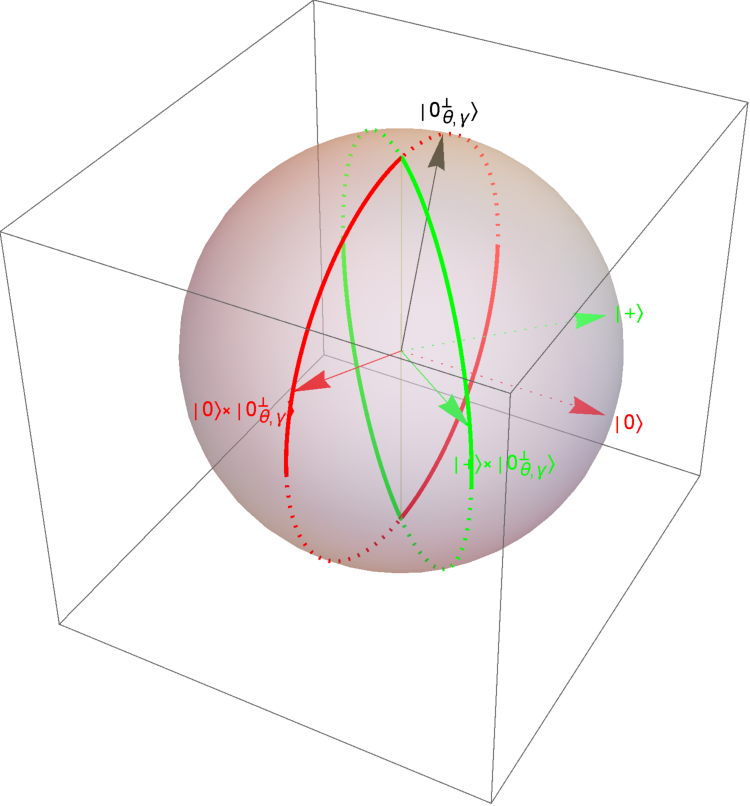
\includegraphics[scale=0.38]{proposal/measure4.pdf}
\end{center}
\caption{\label{fig:three-dimensional-4-value}This figure illustrates
  cases 1 and 2 of example~\ref{ex:three-dimensional-4-value} plotted
  in $\mathbb{R}^{3}$. The red and green dotted vectors are $\ket{0}$
  and $\ket{\ps}$ respectively.  All possible real vectors of the subspaces
  $\ket{0_{\theta,\gamma}^{\perp}}$ and
  $\ket{\ps_{\theta,\gamma}^{\perp}}$ are drawn in the red and green
  circles, respectively. Within the circles, a dotted
  vector~$\ket{\psi}$ means $\bar{\mu}(\proj{\psi})=\likely$;
  otherwise, $\bar{\mu}(\proj{\psi})=\unlikely$. The gray vector is a
  generic vector~$\ket{0_{\theta,\gamma}^{\perp}}$, and the red and
  green solid vectors are normalized
  $\ket{0}\times\ket{0_{\theta,\gamma}^{\perp}}$ and
  $\ket{\ps}\times\ket{0_{\theta,\gamma}^{\perp}}$, respectively, where
  $\times$ is the usual cross product in $\mathbb{R}^{3}$.}
\end{figure}

Looking closely at the example above, we might think that the
probability measure $\bar{\mu}$ is induced by the state $\ket{2}$
because $\bar{\mu}(\proj{0})=\bar{\mu}(\proj{\ps})=\imposs$, or we
might think it is induced by the state $\ket{1}$ because
$\bar{\mu}(\proj{0})=\bar{\mu}(\proj{\ps'})=\imposs$, or yet we might
think it is induced by the mixed state $\frac{\mathbb{1}}{3}$ because
$\bar{\mu}(\proj{\phi})\ne\necess$ for all $\ket{\phi}$. Each of these
possibilities is compatible with some but not all of the
observations. All is not lost however: if the observations are made
more precise, we conjecture that some of the inconsistencies
disappear. A partial proof of this conjecture is the following example
which refines the previous probability measure by adding more precise
intervals. It remains to prove that this refined measure is convex,
however. 

\begin{example}[Three-dimensional quantum four-interval-valued 
  probability measure]\label{ex:three-dimensional-4-value}
  Given a three dimensional Hilbert space with an orthonormal basis
  $\left\{ \ket{0},\ket{1},\ket{2}\right\} $.  Let \emph{
  }$\mathscr{I}=\left\{ \imposs,\unlikely,\likely,\necess\right\} $,
  $\ket{\ps}=\frac{1}{\sqrt{2}}(\ket{0}+\ket{1})$, and
  $\ket{\ms}=\frac{1}{\sqrt{2}}(\ket{0}-\ket{1})$. The definition of
  $\bar{\mu}$ below refers to Fig.~\ref{fig:three-dimensional-4-value}
  which plots the 1-dimensional projectors:
\begin{enumerate}
\item Let:
\begin{eqnarray*}
\bar{\mu}(\mathbb{0})=\bar{\mu}(\proj{0})=\bar{\mu}(\proj{\ps}) 
  &=& \imposs \\
\bar{\mu}(\mathbb{1})=\bar{\mu}(\mathbb{1}-\proj{0})=\bar{\mu}(\mathbb{1}-\proj{\ps}) 
  &=& \necess
\end{eqnarray*}
where $\ket{0}$ and $\ket{\ps}$ are plotted as the red and green dotted
vectors, respectively.
\item The red and green circles are are the states orthogonal to
  $\ket{0}$ and $\ket{\ps}$, respectively, and can be parametrized as
  $\ket{0_{\theta,\gamma}^{\perp}}=\rme^{\rmi\gamma}\sin\theta\ket{1}+\cos\theta\ket{2}$
  and
  $\ket{\ps_{\theta,\gamma}^{\perp}}=-\rme^{\rmi\gamma}\sin\theta\ket{\ms}+\cos\theta\ket{2}$,
  where $0\le\theta\le\frac{\pi}{2}$ and $0\le\gamma<2\pi$. The dotted
  half of those states need special treatment, i.e., whenever
  $0\le\theta<\frac{\pi}{2}$ and $0\le\gamma<\pi$, we define
\begin{eqnarray*}
\bar{\mu}\left(\proj{0_{\theta,\gamma}^{\perp}}\right)=\bar{\mu}\left(\proj{\ps_{\theta,\gamma}^{\perp}}\right)
  &=& \likely \\
\bar{\mu}\left(\mathbb{1}-\proj{0_{\theta,\gamma}^{\perp}}\right)=
  \bar{\mu}\left(\mathbb{1}-\proj{\ps_{\theta,\gamma}^{\perp}}\right) 
  &=& \unlikely
\end{eqnarray*}
\item Otherwise, $\bar{\mu}(\proj{\psi})=\unlikely$ and $\bar{\mu}(\mathbb{1}-\proj{\psi})=\likely$. 
\end{enumerate}
It is straightforward but tedious to check that $\bar{\mu}$ is a
quantum interval-valued probability measure. Although we have not
verified that $\bar{\mu}$ is convex, the following argument
establishes that is has an empty core. Assume there is a real-valued
probability measure satisfying $\mu_{\rho}^{B}(P)\in\bar{\mu}(P)$ for
all $P\in\events$. Because
$\mu_{\rho}^{B}(\proj{0})\in\bar{\mu}(\proj{0})=\imposs$ and
$\mu_{\rho}^{B}(\proj{\ps})\in\bar{\mu}(\proj{\ps})=\imposs$, we must
have $\mu_{\rho}^{B}(\proj{0})=\mu_{\rho}^{B}(\proj{\ps})=0$ so that
$\mu_{\rho}^{B}=\mu_{\ket{2}}^{B}$. However,
\[
\mu_{\ket{2}}^{B}(\proj{2})=1\notin\unlikely=\bar{\mu}(\proj{2})\textrm{ .}
\]
This measure however is ``better'' than the previous one in the sense
that it might only be induced by $\ket{2}$ or the density matrix
$\frac{\mathbb{1}}{3}$, but not by
$\ket{1}$. 
\end{example}

In general, we conjecture that if the measurement equipment is made
more and more precise, the corresponding interval-valued probability
measure will be closer and closer to the Born rule. In the limit case,
$\mathscr{I}=\set{\left\{ a\right\} }{a\in\left[0,1\right]}$ we do
indeed recover the conventional Gleason's theorem and the Born rule.

%%%%%%%%%%%%%%%%%%%%%%%%%%%%%%%%%%%%%%%%%%%%%%%%%%%%%%%%%%%%%%%%%%%%%%%%%%%%%%
\section{Conclusion and Discussion}

If we insist that probabilities cannot be computed to infinite precision
and are bound to be approximations represented by intervals of confidence,
then quantum states themselves can only be discussed within intervals
of confidence. Despite the fact that classically a IVPM could always
correspond to a real-valued probability measure, we found that there
may be no ``real'' infinitely-precise quantum state approximated
by a quantum IVPM as a whole. However, if a quantum IVPM is decomposed
into pieces, each piece might still be induced by a quantum state.
Moreover, our examples and Gleason's theorem summarized in table~\ref{table_long}
suggests that as the measurement resources increase, an entire quantum
IVPM could more and more likely be identified to a particular state.
\begin{table}[ht]
\center{%
\begin{tabular}{c|cccc}
Measurement resources & Lowest & \multicolumn{2}{c}{$\longleftrightarrow$} & Highest\tabularnewline
\hline 
Count of $\mathscr{I}$ & $3$ & $4$ & \ldots{} & $\infty$\tabularnewline
$\sup_{\left[l,r\right]\in\mathscr{I}}\left|r-l\right|$ & $1$ & $\frac{1}{2}$ & \ldots{} & $0$\tabularnewline
Count of $\mathrm{core}\left(\bar{\mu}\right)$ & 0 & 0 &  & 1\tabularnewline
Count of states correspond to pieces of $\bar{\mu}$ & $3$ & $2$ & \ldots{} & $1$\tabularnewline
\hline 
How precise we could identify a state? & Coarse & \multicolumn{2}{c}{$\longleftrightarrow$} & Precise\tabularnewline
\end{tabular}}\caption{Relation between measurement resources and interval-valued probability
measures}
\label{table_long}
\end{table}
Additional work is in progress on the following research questions:
\begin{description}
\item [{Research Question.}] Confirm that there is always a quantum IVPM
with an empty-core if the length of the intervals is bigger than zero. 
\item [{Research Question.}] Find a general method to determine how a
quantum IVPM is close to the Born rule. 
\item [{Research Question.}] Confirm that as the number and precision
of the intervals increase the quantum IVPM converges to the measure
induced by the Born rule. 
\item [{Research Question.}] Investigate the status of the theorems of
Bell and Kochen-Specker for quantum IVPM.
\end{description}
Although we discussed how a quantum IVPM could be induced from a real
quantum state, our investigation leaves an open question of whether
there exists a ``real'' entity that exists independently of measurements
and probabilities. The possibility of no ``real'' underlying state
is consistent with the elegantly recent work on Quantum Bayesianism
or QBism~\cite{Fuchs2010,VonBaeyer2016,Fuchs2012}, which suggests
that the quantum state is more like an interactive system in computer
science parlance. In another word, the quantum state is subjective:
each observer has a different view of the quantum system that is consistent
with their previous observations and that allows that observer, independently
of other observers, to assign beliefs (i.e., probabilities) to possible
future interactions.

%%%%%%%%%%%%%%%%%%%%%%%%%%%%%%%%%%%%%%%%%%%%%%%%%%%%%%%%%%%%%%%%%%%%%%%%%%%%%%
\newpage{}%
\begin{comment}
 \bibliographystyle{plain}
\bibliography{proposal/prop}
 
\end{comment}
\printbibliography

\appendix

\section{Increasing the Measurement Resource}

Although quantum IVPMs in example~\ref{ex:three-dimensional-three-value}
and \ref{ex:three-dimensional-4-value} have empty cores, we might
still think that the probability measure~$\bar{\mu}$ is induced
by some states. In example~\ref{ex:three-dimensional-three-value},
the probability measure~$\bar{\mu}$ might be induced by the state
$\ket{2}$ because $\bar{\mu}(\proj{0})=\bar{\mu}(\proj{\ps})=\imposs$,
or induced by the state $\ket{1}$ because $\bar{\mu}(\proj{0})=\bar{\mu}(\proj{\ps'})=\imposs$.
In example~\ref{ex:three-dimensional-4-value}, the probability measure~$\bar{\mu}$
might be induced by the state $\ket{2}$ because $\bar{\mu}(\proj{0})=\bar{\mu}(\proj{\ps})=\imposs$.
In general, each two real 1-dimensional projectors~$\proj{\psi_{0}}$
and $\proj{\psi_{1}}$ mapping to impossible suggests $\bar{\mu}$
might be induced by the pure state~$\ket{\psi_{0}}\times\ket{\psi_{1}}$
in the Hilbert space of dimension 3.

Since a quantum IVPM is completely determined by its value on 1-dimensional
projectors in the Hilbert space of dimension 3, we could define the
interval-valued frame function to simplify the later discussion.

\begin{definition}\cite{Hatcher2001,dryden2005}~The unit sphere
in $\mathbb{R}^{d}$ is denoted by $S^{d-1}=\set{\ket{\psi}\in\mathbb{R}^{d}}{\ip{\psi}{\psi}=1}$,
while the unit sphere in $\mathbb{C}^{d}$ is denoted by $\mathbb{C}S^{d-1}=\set{\ket{\psi}\in\mathbb{C}^{d}}{\ip{\psi}{\psi}=1}$.
Since $\mathbb{C}$ is one-to-one correspondence to $\mathbb{R}^{2}$~\cite{GAMELIN2003},
$\mathbb{C}S^{d-1}$ has the same structure as $S^{2d-1}$. However,
different symbols emphasis that they are embedded in different spaces.\end{definition}

\begin{definition}\cite{gleason1957,peres1995quantum,RichmanBridges1999}~For
any quantum probability measure~$\mu$ on the Hilbert space of dimension
3, we can define its \emph{frame function}~$f:\mathbb{C}S^{2}\rightarrow\left[0,1\right]$
by $f\left(\ket{\psi}\right)=\mu\left(\proj{\psi}\right)$. For a
quantum probability measure~$\mu_{\phi}^{B}$ induced by the Born
rule, its frame function is denoted by $f_{\phi}^{B}$.\end{definition}

\begin{lemma}\cite{gleason1957,peres1995quantum,RichmanBridges1999}~A
frame function~$f:\mathbb{C}S^{2}\rightarrow\left[0,1\right]$ satisfies
the following properties:
\begin{itemize}
\item $f\left(\lambda\ket{\psi}\right)=f\left(\ket{\psi}\right)$ for any
$\ket{\psi}\in\mathbb{C}S^{2}$ and $\lambda\in\mathbb{C}S^{0}$.
\item For any orthonormal basis~$\left\{ \ket{\psi_{i}}\right\} _{i=0}^{2}$,
we have $1=\sum_{i=0}^{2}f\left(\ket{\psi_{i}}\right)$.
\end{itemize}
Conversely, if a function~$f:\mathbb{C}S^{2}\rightarrow\left[0,1\right]$
satisfies the above properties, $f$ must be a frame function.\end{lemma}

\begin{definition}For any quantum IVPM~$\bar{\mu}$ on the Hilbert
space of dimension 3, we can define an \emph{interval-valued frame
function}~$\bar{f}:\mathbb{C}S^{2}\rightarrow\mathscr{I}$ by $\bar{f}\left(\ket{\psi}\right)=\bar{\mu}\left(\proj{\psi}\right)=\left[f^{l}\left(\ket{\psi}\right),f^{r}\left(\ket{\psi}\right)\right]$,
where $f^{l}:\mathbb{C}S^{2}\rightarrow\left[0,1\right]$ and $f^{r}:\mathbb{C}S^{2}\rightarrow\left[0,1\right]$
are the left-end and the right-end of $\bar{f}$, respectively. Also,
if $f$ is the frame function of $\mu$, $\bar{f}$ is the interval-valued
frame function of $\bar{\mu}$, and $\mu$ is in the core of $\bar{\mu}$,
then we say $f$ is in the core of $\bar{f}$, and denoted by $f\in\mathrm{core}\left(\bar{f}\right)$.\end{definition}

\begin{lemma}A interval-valued frame function~$\bar{f}:\mathbb{C}S^{2}\rightarrow\mathscr{I}$
satisfies the following properties:
\begin{itemize}
\item $\bar{f}\left(\lambda\ket{\psi}\right)=\bar{f}\left(\ket{\psi}\right)$
for any $\ket{\psi}\in\mathbb{C}S^{2}$ and $\lambda\in\mathbb{C}S^{0}$.
\item For any orthonormal basis~$\left\{ \ket{\psi_{i}}\right\} _{i=0}^{2}$,
we have $1\in\sum_{i=0}^{2}\bar{f}\left(\ket{\psi_{i}}\right)$ and
$\left[1,1\right]-\bar{f}\left(\ket{\psi_{i}}\right)\subseteq\bar{f}\left(\ket{\psi_{j}}\right)+\bar{f}\left(\ket{\psi_{k}}\right)$,
where $i$, $j$, and $k$ are any permutations among $0$, $1$,
and $2$.
\end{itemize}
Conversely, if a function~$\bar{f}:\mathbb{C}S^{2}\rightarrow\mathscr{I}$
satisfies the above properties, $\bar{f}$ must be an interval-valued
frame function.\end{lemma}
\begin{proof}
Given a quantum IVPM~$\bar{\mu}$, it is straightforward to verify
that its interval-valued frame function~$\bar{f}:\mathbb{C}S^{2}\rightarrow\mathscr{I}$
satisfies the above properties.

Conversely, given a function~$\bar{f}:\mathbb{C}S^{2}\rightarrow\mathscr{I}$
satisfying the above properties, consider $\bar{\mu}:\events\rightarrow\mathscr{I}$
defined by
\begin{itemize}
\item $\bar{\mu}(\mathbb{0})=\left[0,0\right]$ and $\bar{\mu}(\mathbb{1})=\left[1,1\right]$. 
\item For any $\ket{\psi}\in\mathbb{C}S^{2}$, we have $\bar{\mu}\left(\proj{\psi}\right)=\bar{f}\left(\ket{\psi}\right)$
and $\bar{\mu}\left(\mathbb{1}-\proj{\psi}\right)=\left[1,1\right]-\bar{f}\left(\ket{\psi}\right)$.
\end{itemize}
Since other conditions are trivial, we only need to verify 
\begin{equation}
\bar{\mu}\left(\sum_{i=1}^{N}P_{i}\right)\subseteq\sum_{i=1}^{N}\bar{\mu}\left(P_{i}\right)\label{eq:quantumIVPMconditions}
\end{equation}
 for any set of mutually orthogonal projections $\left\{ P_{i}\right\} _{i=1}^{N}$.
First, if $\mathbb{0}$ or $\mathbb{1}$ is in $\left\{ P_{i}\right\} _{i=1}^{N}$,
the statement could be reduced to the case without $\mathbb{0}$,
or its trivial. Hence, we only need to discuss $\left\{ P_{i}\right\} _{i=1}^{N}$
containing 1- or 2-dimensional projectors. When $\left\{ P_{i}\right\} _{i=1}^{N}$
containing a 2-dimensional projector, the definition of $\bar{\mu}$
implies equation~(\ref{eq:quantumIVPMconditions}). When $\left\{ P_{i}\right\} _{i=1}^{N}$
only containing 1-dimensional projectors, the properties of $\bar{f}$
implies equation~(\ref{eq:quantumIVPMconditions}).
\end{proof}
\begin{definition}For $\ket{\psi}=\alpha_{0}\ket{0}+\alpha_{1}\ket{1}+\alpha_{2}\ket{2}=\begin{pmatrix}\alpha_{0}\\
\alpha_{1}\\
\alpha_{2}
\end{pmatrix}$ and $\ket{\phi}=\beta_{0}\ket{0}+\beta_{1}\ket{1}+\beta_{2}\ket{2}=\begin{pmatrix}\beta_{0}\\
\beta_{1}\\
\beta_{2}
\end{pmatrix}$, their cross product is defined as follow: 
\[
\ket{\psi\times\phi}=\ket{\psi}\times\ket{\phi}=\begin{vmatrix}\alpha_{1}^{*} & \beta_{1}^{*}\\
\alpha_{2}^{*} & \beta_{2}^{*}
\end{vmatrix}\ket{0}+\begin{vmatrix}\alpha_{2}^{*} & \beta_{2}^{*}\\
\alpha_{0}^{*} & \beta_{0}^{*}
\end{vmatrix}\ket{1}+\begin{vmatrix}\alpha_{0}^{*} & \beta_{0}^{*}\\
\alpha_{1}^{*} & \beta_{1}^{*}
\end{vmatrix}\ket{2}\textrm{ ,}
\]
where $\begin{vmatrix}\alpha & \beta\\
\alpha' & \beta'
\end{vmatrix}=\alpha\beta'-\alpha'\beta$. Also, even if $\ket{\psi}$ and $\ket{\phi}$ are normalized, their
cross product~$\ket{\psi}\times\ket{\phi}$ need not be normalized
as usual. We will use $\ket{\psi}\times\ket{\phi}$ and $\frac{\ket{\psi}\times\ket{\phi}}{\left\Vert \ket{\psi}\times\ket{\phi}\right\Vert }$
interchanged when there is no confusion.\end{definition}

\begin{definition}For $\ket{\psi}$ and $\ket{\phi}\in\mathbb{C}^{3}$,
if $\ket{\psi}=\lambda\ket{\phi}$ for some~$\lambda\ne0$, we call
$\ket{\psi}$ is parallel to $\ket{\phi}$ denoted by $\ket{\psi}\parallel\ket{\phi}$.
In this case, $\ket{\psi}$ and $\ket{\phi}$ represent the same physical
state. ``$\ket{\psi}$ is not parallel to $\ket{\phi}$'' is denoted
by $\ket{\psi}\nparallel\ket{\phi}$.\end{definition}

\begin{lemma}Given $\ket{\psi}$, $\ket{\phi}$ and $\ket{\varphi}\in\mathbb{C}^{3}$
such that $\ket{\psi}\nparallel\ket{\phi}$. Then, $\ket{\varphi}\parallel\left(\ket{\psi}\times\ket{\phi}\right)$
if and only if $\ip{\psi}{\varphi}=\ip{\phi}{\varphi}=0$.\end{lemma}
\begin{proof}
To prove that $\ket{\varphi}\parallel\left(\ket{\psi}\times\ket{\phi}\right)\Rightarrow\ip{\psi}{\varphi}=\ip{\phi}{\varphi}=0$,
we can just verify 
\begin{eqnarray*}
\ip{\psi}{\psi\times\phi} & = & \ip{\psi\times\phi}{\psi}^{*}=\left[\left(\alpha_{1}\beta_{2}-\alpha_{2}\beta_{1}\right)\alpha_{0}+\left(\alpha_{2}\beta_{0}-\alpha_{0}\beta_{2}\right)\alpha_{1}+\left(\alpha_{0}\beta_{1}-\alpha_{1}\beta_{0}\right)\alpha_{2}\right]^{*}=0\textrm{ ,}\\
\ip{\phi}{\psi\times\phi} & = & \ip{\psi\times\phi}{\phi}^{*}=\left[\left(\alpha_{1}\beta_{2}-\alpha_{2}\beta_{1}\right)\beta_{0}+\left(\alpha_{2}\beta_{0}-\alpha_{0}\beta_{2}\right)\beta_{1}+\left(\alpha_{0}\beta_{1}-\alpha_{1}\beta_{0}\right)\beta_{2}\right]^{*}=0\textrm{ .}
\end{eqnarray*}

To prove the other direction, consider the linear transformation~$T:\mathbb{C}^{3}\rightarrow\mathbb{C}^{2}$
defined by $T\left(\ket{\varphi}\right)=\begin{pmatrix}\ip{\psi}{\varphi}\\
\ip{\phi}{\varphi}
\end{pmatrix}$. Since $\ket{\psi}\nparallel\ket{\phi}$, we have $\mathrm{rank}\left(T\right)=2$.
Together with the rank equation~\cite{FraleighBeauregard1995}, we
have
\[
\dim\left(\ker T\right)=\mathrm{nullity}\left(T\right)=3-\mathrm{rank}\left(T\right)=3-2=1\textrm{ .}
\]
By the other direction of the proof, we have already known $\ket{\psi}\times\ket{\phi}\in\ker T$.
Therefore, $\ket{\varphi}\parallel\left(\ket{\psi}\times\ket{\phi}\right)$.
\end{proof}
Since interval-valued probability measures~$\bar{\mu}$ and interval-valued
frame functions~$\bar{f}$ are one-to-one correspondence, studying
1-dimensional projectors mapping to impossible by $\bar{\mu}$ is
the same as studying the points on $\mathbb{C}S^{2}$ mapping to impossible
by $\bar{f}$. These points, denoted by $\bar{f}^{-1}\left(\imposs\right)=\set{\ket{\psi}\in\mathbb{C}^{3}}{\bar{f}(\ket{\psi})=\imposs}$,
play an important role to understand $\bar{f}$. There are 4 different
cases when analyzing $\bar{f}^{-1}\left(\imposs\right)$:
\begin{enumerate}
\item $\bar{f}^{-1}\left(\imposs\right)=\emptyset$. If $f_{\phi}^{B}\in\mathrm{core}\left(\bar{f}\right)$
for some pure state~$\ket{\phi}$, we could say nothing about $\ket{\phi}$.
\item $\bar{f}^{-1}\left(\imposs\right)=\left\{ \ket{\psi_{0}}\right\} $.
If $f_{\phi}^{B}\in\mathrm{core}\left(\bar{f}\right)$ for some pure
state~$\ket{\phi}$, $\ket{\phi}$ could be any state orthogonal
to $\ket{\psi_{0}}$.
\item Consider $\left\{ \ket{\psi_{0}},\ket{\psi_{1}}\right\} \subseteq\bar{f}^{-1}\left(\imposs\right)$.
If $\left(\ket{\psi_{0}}\times\ket{\psi_{1}}\right)\parallel\left(\ket{\psi_{0}'}\times\ket{\psi_{1}'}\right)$
for any $\left\{ \ket{\psi_{0}'},\ket{\psi_{1}'}\right\} \subseteq\bar{f}^{-1}\left(\imposs\right)$,
then $\ket{\psi_{0}}\times\ket{\psi_{1}}$ is the only pure state
which might induce $\bar{f}$. In another word, if $f_{\phi}^{B}\in\mathrm{core}\left(\bar{f}\right)$
for some pure state~$\ket{\phi}$, then $\ket{\phi}\parallel\left(\ket{\psi_{0}}\times\ket{\psi_{1}}\right)$. 
\item If another pair of states~$\ket{\psi_{0}'}$ and $\ket{\psi_{1}'}\in\bar{f}^{-1}\left(\imposs\right)$
gives different state of cross product~$\ket{\psi_{0}'}\times\ket{\psi_{1}'}$,
then both $\ket{\psi_{0}}\times\ket{\psi_{1}}$ and $\ket{\psi_{0}'}\times\ket{\psi_{1}'}$
might induce $\bar{f}$, but neither $f_{\ket{\psi_{0}}\times\ket{\psi_{1}}}^{B}$
nor $f_{\ket{\psi_{0}'}\times\ket{\psi_{1}'}}^{B}$ in the core of
$\bar{f}$ because $f_{\ket{\psi_{0}}\times\ket{\psi_{1}}}^{B}$ is
inconsistent with $\bar{f}(\proj{\psi_{0}'})=\bar{f}(\proj{\psi_{1}'})=\imposs$
and $f_{\ket{\psi_{0}'}\times\ket{\psi_{1}'}}^{B}$ is inconsistent
with $\bar{f}(\proj{\psi_{0}})=\bar{f}(\proj{\psi_{1}})=\imposs$.
Actually, $\bar{f}$ has an empty core. 
\end{enumerate}
In summary, if we have an idea of $\bar{f}^{-1}\left(\imposs\right)$,
we could have some idea of the pure states in core.

As we did in Fig.~\ref{fig:three-dimensional-4-value}, we could
plot the 1-dimensional projectors in a unit sphere~$S^{2}$~\cite{Hatcher2001,dryden2005}.
Since the state mapping to impossible always contained in a plane,
$\bar{f}^{-1}\left(\imposs\right)$ in the above case 2 - 4 does not
contain any area in $S^{2}$. In contrast, if $\bar{f}^{-1}\left(\imposs\right)$
contains some area in $S^{2}$, it must be the situation of case 1.
Furthermore, the larger the area, the more 1-dimensional projectors
which is inconsistent with any particular Born rule probability measure.
Therefore, the area of $\bar{f}^{-1}\left(\imposs\right)$ could indicate
how much $\bar{f}$ deviate from the Born rule probability measures.\footnote{Notice that we only discuss only discuss real 1-dimensional projectors
in the Hilbert space of dimension 3. In general, we could discuss
all 1-dimensional projectors in any dimension. However, restricting
to $\mathbb{R}^{3}$ enable us to use cross product which will simplify
our discussion a lot, and $\mathbb{R}^{3}$ is easy to visualize and
imagine. Also, if a quantum IVPM~$\bar{\mu}$ has an empty core when
restricting to $\mathbb{R}^{3}$, $\bar{\mu}$ has an empty core on
the original space as well. So restricting on real 1-dimensional projectors
still provides valid results.}

In order to simplify the discussion, let's set the center of $\bar{f}^{-1}\left(\imposs\right)$
as the north pole, and assume $\bar{f}$ maps every state whose latitude
is larger than $\theta_{0}$ to impossible. In order to simplify the
notation, let's give the following definition.

\begin{definition}Given a vector~$\ket{\psi}\in S^{2}$ with a specified
north pole~$\ket{0}\in S^{2}$, then $\theta\left(\ket{\psi}\right)=\arccos\ip{0}{\psi}$
denotes the the latitude of $\ket{\psi}$.\end{definition}

\section{Subset of Commuting Events}

\footnote{\yutsung{The Kochen-Specker theorem is about assigning definitely
value to observables such that the values of commuting observables
are consistent; the Bell theorem is about entangled states in different
locations. If our results are more related to commuting observables,
it is more related to the Kochen-Specker theorem than the Bell theorem...}}

Given an orthonormal basis~$\mathcal{B}=\left\{ \ket{\psi_{1}},\ldots,\ket{\psi_{d}}\right\} $
of a Hilbert space, the set of projections generated by the basis
is $\events'=\set{\sum_{\ket{\psi}\in S}\ket{\psi}}{S\subseteq\mathcal{B}}$.
Because $\left(2^{\mathcal{B}},\emptyset,\mathcal{B},\cup,\cap\right)$
is isomorphic to $\left(\events',\mathbb{0},\mathbb{1},\vee,\cdot\right)$
as a Boolean algebra, a quantum IVPM~$\bar{\mu}':\events'\rightarrow\mathscr{I}$
is essentially a classical IVPM~$\bar{\mu}:2^{\mathcal{B}}\rightarrow\mathscr{I}$.
By the Shapley theorem, if $\bar{\mu}'$ is convex, it should have
a non-empty core. 

The problem is: if $\events'$ is only a commuting subset of $\events$,
does a convex quantum IVPM~$\bar{\mu}':\events'\rightarrow\mathscr{I}$
always has a non-empty core?

\end{document}

%%%%%%%%%%%%%%%%%%%%%%%%%%%%%%%%%%%%%%%%%%%%%%%%%%%%%%%%%%%%%%%%%%%%%%%%%%%%%%



